% Auto-ABM paper draft for EMNLP 2026 System Demonstrations.
% Compile from papers/rest:
%   pdflatex main
%   bibtex main
%   pdflatex main
%   pdflatex main

\documentclass[11pt]{article}

\usepackage[preprint]{acl}
\usepackage{times}
\usepackage{latexsym}
\usepackage[T1]{fontenc}
\usepackage[utf8]{inputenc}
\usepackage{microtype}
\usepackage{inconsolata}
\usepackage{graphicx}
\usepackage{booktabs}
\usepackage{tabularx}
\usepackage{array}
\usepackage{xcolor}
\usepackage{enumitem}

\newcommand{\sys}{Auto-ABM}
\newcolumntype{Y}{>{\raggedright\arraybackslash}X}

\title{\sys: A Simulation-First Workbench for Trace-Grounded Agent-Based Modeling\thanks{Project repository: \url{https://github.com/ShuhanLexX/Auto-ABM}. Product release: \url{https://github.com/ShuhanLexX/Auto-ABM/releases/tag/v1.0.0}.}}

\author{Shuhan Zhang \\
  School of Law, Zhengzhou University \\
  Zhengzhou, Henan, China \\
  \texttt{z1811744767@163.com}}

\begin{document}
\maketitle

\begin{abstract}
Agent-based modeling (ABM) studies how system-level patterns emerge from the local decisions of interacting agents. As ABM has become a central method for computational social science, epidemiology, economics, and complex-systems research, its practical burden has also grown: researchers spend substantial time turning hypotheses into executable models, running and comparing simulations, tracing mechanisms, and packaging reproducible evidence. Large language models can accelerate programming, yet many ABM workflows still leave assumptions, traces, explanations, experiments, and exports outside the same research loop. We present \sys{}, to our knowledge the first AI-native, simulation-first workbench for ABM research. \sys{} organizes specialized research agents around a versioned simulation object backed by a deterministic Mesa kernel and a trace ledger. It supports mechanism proposal, model formalization, execution, trace-grounded explanation, adaptive experimentation, and ODD-aligned export in one workflow. Across a planned benchmark of eight ABM task families, draft pilot estimates indicate higher averaged scores for executability, mechanism validity, evidence grounding, experimental design, and reproducible reporting than code-centered baselines.
\end{abstract}

\section{Introduction}

Agent-based modeling is a powerful methodology for studying systems in which macro-level patterns emerge from local interactions among heterogeneous agents \citep{bonabeau2002abm,macal2010tutorial}. Its appeal has increased as researchers seek models that can express adaptation, spatial structure, network effects, and policy interventions without collapsing them into a single closed-form equation. Yet ABM remains labor-intensive. A typical study must turn a research question into mechanisms, encode those mechanisms in a simulator, validate assumptions, compare runs, interpret traces, and document the model in a form that another researcher can inspect.

Recent tools can generate simulator code or assist with a particular modeling environment. This lowers the programming barrier, but it rarely changes the organization of the research object itself. The executable script still becomes the center of gravity. Traces, ODD descriptions, explanations, experiment plans, and reproduction bundles are often assembled after the run, which makes it difficult to audit how a claim about emergent behavior was produced.

\sys{} starts from a different premise. In ABM research, the durable object is not a script but a versioned simulation: a bundle of assumptions, parameters, runs, traces, explanations, experiments, and exportable evidence. The system treats language models as research collaborators whose actions are constrained by this object. A hypothesis agent proposes candidate mechanisms, a modeling agent formalizes the selected candidate, an execution agent delegates runs to a deterministic kernel, an evidence agent reads trace intervals, an experiment agent designs sweeps or interventions, and a documentation agent maintains ODD-aligned descriptions. These roles cooperate through the trace ledger, so explanatory language is downstream of executable evidence.

This paper contributes:
\begin{itemize}[leftmargin=*]
  \item a simulation-first workflow for LLM-assisted ABM that keeps model structure, execution traces, explanations, experiments, and export artifacts linked throughout a research session;
  \item a multi-agent orchestration protocol in which specialized research roles coordinate through versioned simulation objects rather than through arbitrary code edits;
  \item a trace-grounded explanation mechanism that separates deterministic analytics from natural-language narration and verifies cited facts against the selected run interval;
  \item an AI-native software system that integrates mechanism proposal, model execution, explanation, experimentation, and ODD-aligned export inside one ABM research workbench.
\end{itemize}

\section{Related Work}

ABM has long been used to study complex adaptive systems by specifying local rules and observing emergent population-level behavior \citep{bonabeau2002abm,macal2010tutorial}. Classic families such as segregation, epidemic spread, threshold cascades, innovation diffusion, opinion dynamics, cooperation, and forest-fire spread provide reusable testbeds for modeling assumptions \citep{schelling1971segregation,kermack1927epidemics,granovetter1978threshold,bass1969new,deffuant2000mixing,nowak2006five,drossel1992forest}. Toolkits such as NetLogo \citep{wilensky1999netlogo} and Mesa \citep{kazil2020mesa,terhoeven2025mesa3} make these models executable, while the ODD protocol standardizes model description and supports replication \citep{grimm2020odd}. \sys{} builds on this tradition by making the simulation object, not the surrounding code, the unit that the conversational system creates, revises, runs, and exports.

Recent systems use LLMs to assist simulation authoring, including NetLogo-oriented assistants and verifier-assisted ABM code generation \citep{chen2024netlogochat,martinez2024netlogo,niu2024sage}. These systems show that language models can help users translate natural-language scenarios into executable models, but they generally focus on model construction rather than on the full evidence lifecycle of ABM research. A broader line of work studies agentic language-model systems that interleave reasoning and tool use \citep{yao2023react}. \sys{} adopts this general pattern, but constrains it to ABM-specific research roles and evidence objects. Its central distinction is that generated explanations, charts, and experiments are resolved against recorded simulation traces, providing a stronger provenance boundary than free-form code generation alone.

\section{System Overview}
\label{sec:system}

\sys{} is a desktop research workbench for ABM. Its central abstraction is a versioned simulation rather than a generated program. A project contains one or more simulations, and each simulation binds the model specification, ODD document, interface state, run records, traces, experiment plans, explanations, and export artifacts. The abstraction follows the ABM view that macro patterns arise from local agent rules \citep{bonabeau2002abm,macal2010tutorial}, while making intermediate evidence inspectable during routine modeling.

\begin{figure*}[t]
  \centering
  \begin{tabular}{@{}cc@{}}
    \screenplaceholder{Research Workspace}{Conversation, proposal batch, and selected simulation state.} &
    \screenplaceholder{Simulation Canvas}{Spatial run view, metric panel, and trace-linked inspection.} \\[0.8em]
    \screenplaceholder{Mechanism Atlas}{Mechanism graph, attribution path, and explanation evidence.} &
    \screenplaceholder{Experiment Workspace}{Sweep controls, intervention setup, and resolved result panels.}
  \end{tabular}
  \caption{System overview placeholder. The camera-ready version will replace these boxes with four screenshots from the current \sys{} workbench, covering the research workspace, simulation canvas, mechanism atlas, and experiment workspace.}
  \label{fig:system-overview}
\end{figure*}

\subsection{Design Principles}
\label{subsec:principles}

Four principles shape the system. First, \sys{} is simulation-centered: the user creates, revises, runs, and exports simulations, while code remains an implementation detail. Second, the trace is the source of truth. Metrics, events, mechanism firings, and spatial snapshots are written as run evidence and reused by charts, explanations, and export. Third, the executable core is deterministic; a run is identified by its model version, seed, parameter snapshot, and kernel version. Fourth, language generation is evidence-constrained. The LLM may summarize or narrate, but cited ticks, metrics, mechanisms, and events must appear in the trace slice supplied by the system.

The system also uses the ODD protocol as a documentation spine \citep{grimm2020odd}. An ODD document is derived from the model configuration and remains linked to the model version. When a user changes model structure, \sys{} updates the ODD draft and preserves user-authored text when possible. This makes model description a live part of the workflow rather than a final write-up step.

\subsection{Architecture}
\label{subsec:architecture}

\sys{} has three conceptual layers. The interaction layer presents conversation, simulation views, trace explanation, experiment controls, and ODD documentation. The coordination layer maintains versioned project state, mediates role-specific actions, and records provenance for runs and exports. The kernel layer is a Python package built on Mesa \citep{kazil2020mesa,terhoeven2025mesa3}. It executes formal model specifications, emits trace records, derives mechanism graphs, and evaluates batch experiments. This separation keeps the interface responsive without allowing visualization state to become the source of model behavior.

\begin{figure*}[t]
  \centering
  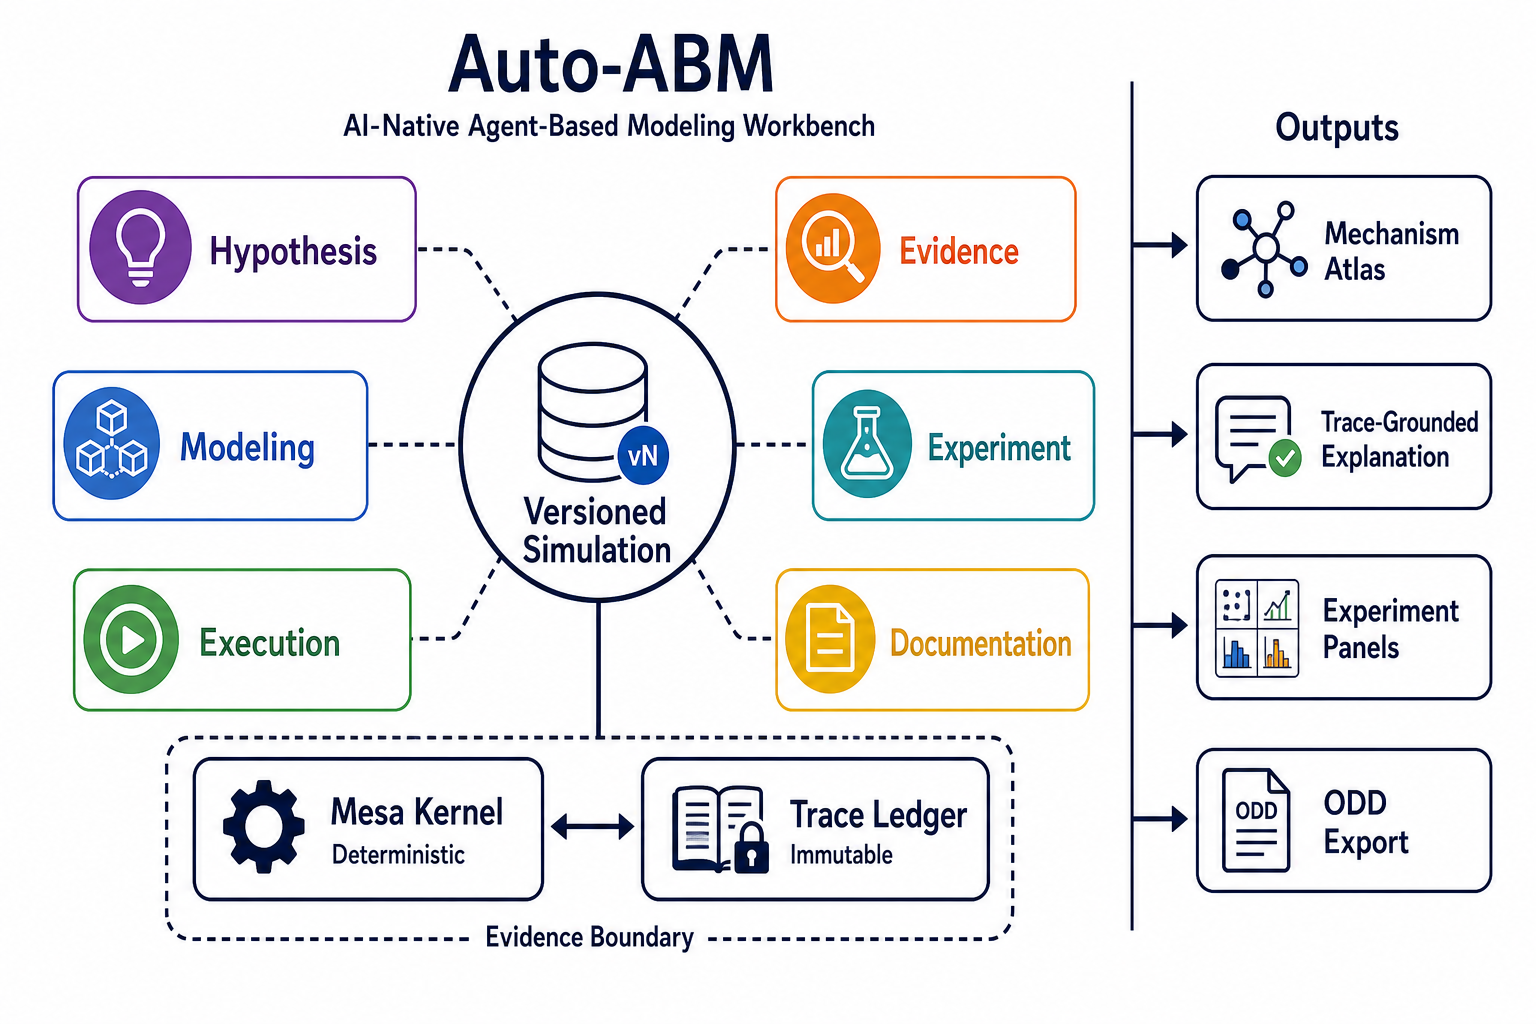
\includegraphics[width=0.98\textwidth]{figures/fig-method-framework-ai.png}
  \caption{Method architecture of \sys{}. Specialized research agents operate over a shared versioned simulation object. The deterministic Mesa kernel and trace ledger define the evidence boundary for mechanism visualization, explanation, experiment analysis, ODD updates, and reproducible export.}
  \label{fig:method-framework}
\end{figure*}

\subsection{End-to-End Data Flow}
\label{subsec:dataflow}

A typical session begins with a research question. The hypothesis agent proposes candidate mechanisms, each paired with expected macro behavior and an ODD-oriented rationale. After the user selects a candidate, the modeling agent formalizes it as a simulation specification and the execution agent records a versioned run. The user can then change parameters, inspect agents, select trace intervals, request explanations, configure experiments, and export a reproduction package. Figure~\ref{fig:method-framework} shows this shared path across forward and inverse research use cases.

Forward and inverse research paths share the same trace layer. In a forward path, the user starts from a mechanism hypothesis and inspects the resulting macro behavior. In an inverse path, the user starts from a target phenomenon and asks the system to propose candidate mechanisms. In both cases, claims about model behavior are grounded in real runs and trace records, not in free-form model output.

\section{Methods}
\label{sec:methods}

\subsection{Research Lifecycle at a Glance}
\label{subsec:lifecycle}

The current system implements a six-stage lifecycle from mechanism drafting to reproducible export. The key design choice is to assign each phase to a research role with a restricted evidential responsibility. The roles cooperate through persistent simulation objects rather than through unstructured edits to source code. Appendix~\ref{app:lifecycle} provides the full lifecycle table.

\subsection{Simulation-Centered Multi-Agent Orchestration}
\label{subsec:workflow}

\textbf{Role specialization.} \sys{} follows the agentic pattern of interleaving reasoning with external action \citep{yao2023react}, but its action space is organized around ABM research roles. The hypothesis agent expands the search space by proposing alternative mechanism families for the same phenomenon. The modeling agent narrows this space by converting an adopted proposal into an explicit specification with agent types, state variables, environment assumptions, mechanisms, observables, and initial conditions. The execution agent submits the specification to the deterministic kernel and records version, seed, parameter snapshot, and run provenance.

\textbf{Evidence handoff.} Downstream roles operate only after a run exists. The evidence agent transforms a selected trace interval into mechanism activity, state-transition attribution, changepoints, and counterfactual comparisons. The language narrator receives this structured evidence packet, not an open-ended invitation to invent measurements. The experiment agent designs parameter sweeps or scheduled interventions and binds result views to stored run records. Finally, the documentation agent updates the ODD narrative and prepares a reproduction package. The same trace interval can therefore appear in the chart, mechanism atlas, attribution view, and explanation text without duplicating the evidential source.

The workbench supports three operating modes. Research mode permits modeling and experiments while requiring confirmation for structural model edits, large batches, overwrites, and export operations. Dialogue mode is read-only: the agents may inspect existing simulations and explain evidence, but they cannot mutate the research object. Autonomous exploration mode chains proposal, short trial runs, ranking, and reporting for unattended exploration; the evaluation in this paper focuses on research mode because it is the end-to-end workflow most directly comparable to existing modeling assistance.

Candidate simulations are generated as diverse mechanism drafts and then mapped to executable families. The current library includes epidemic diffusion, segregation, wildfire, bounded-confidence opinion, innovation diffusion, public-goods cooperation, threshold influence, and platform rumor moderation. Each specification is declarative: it states the agents, state variables, environment parameters, mechanisms, observables, initialization assumptions, and interface defaults. As a result, model assumptions remain inspectable even when they are proposed through natural language.

\subsection{Mechanism Atlas and Trace-Grounded Explanation}
\label{subsec:explain}

The most important methodological choice is to split explanation into two layers. The first layer is deterministic. Given a model configuration, the kernel derives a mechanism graph whose nodes represent agent types, state variables, parameters, mechanisms, and observers. Its edges correspond to explicit structural links or literal references in the configuration. A graph edge is therefore a record of model structure rather than an LLM-generated causal claim.

The second layer reads the run trace. A trace contains metric observations, events, mechanism firings, and, when requested, space snapshots. The coordination layer computes three kinds of trace analytics. Mechanism activity counts which mechanisms fired during an interval. Attribution maps an observed metric to an agent state and decomposes the metric change into signed state-transition flows by mechanism. Changepoint detection scans metric series for salient slope changes. Counterfactual runs reuse the same model version and seed while changing parameters or scheduled interventions, then compare trajectories.

\begin{figure*}[t]
  \centering
  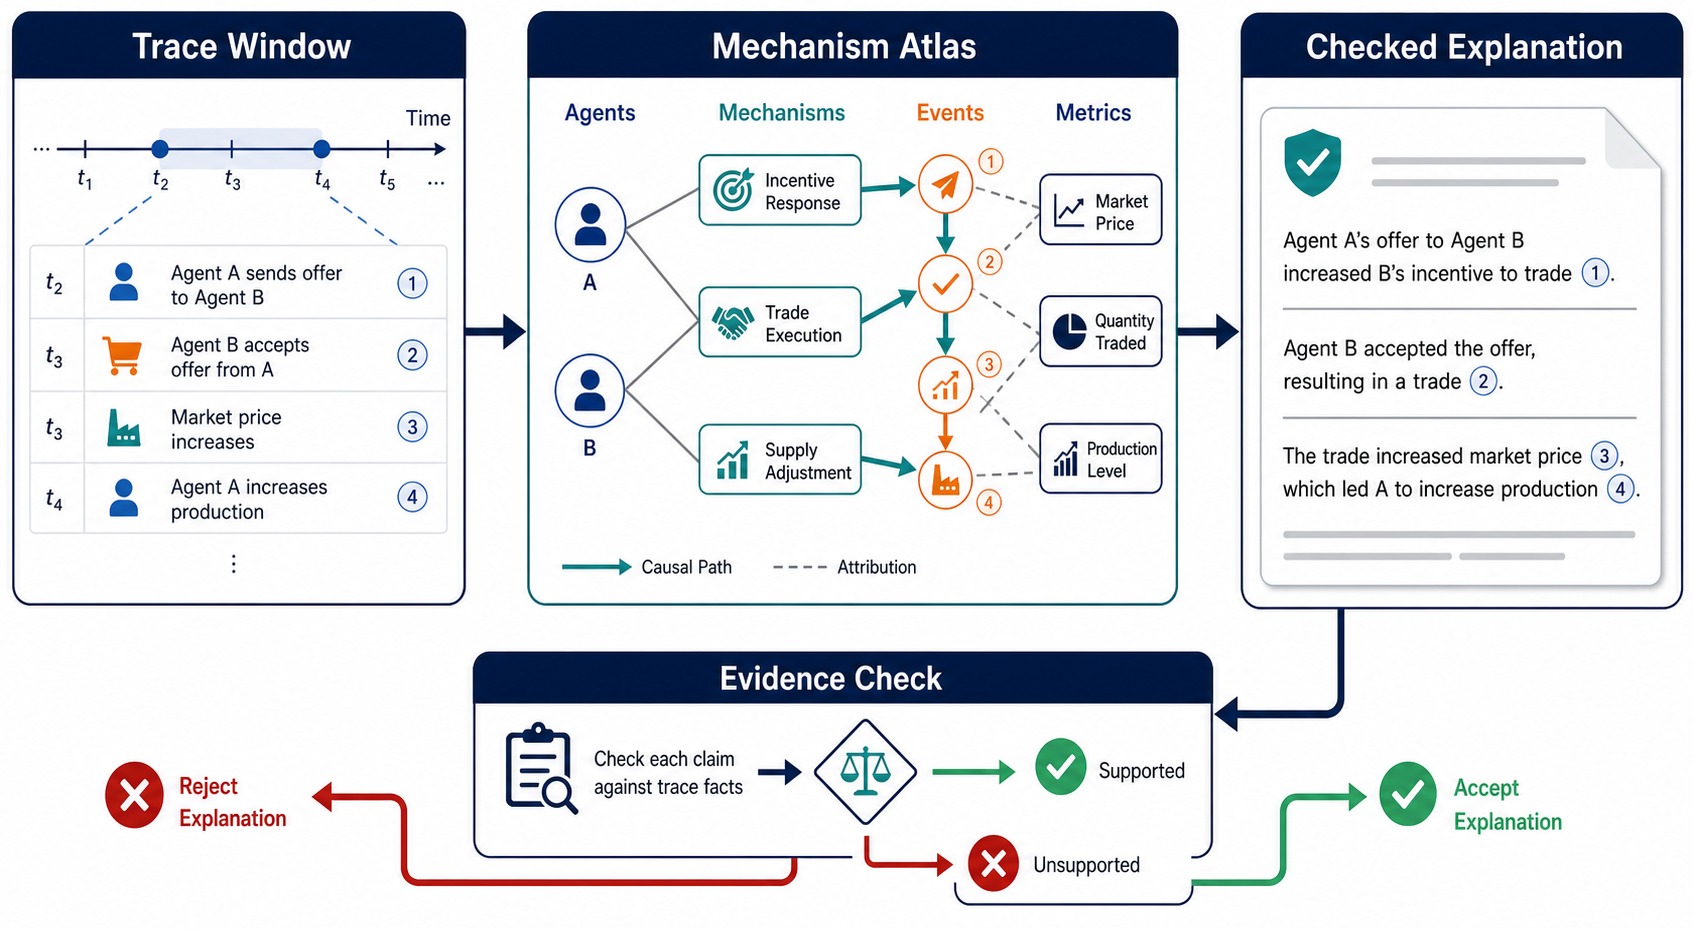
\includegraphics[width=0.98\textwidth]{figures/fig-mechanism-atlas-ai.png}
  \caption{Mechanism atlas and trace-grounded explanation. The system links a selected trace window to mechanism paths, attribution evidence, and checked explanatory statements. Unsupported claims are rejected by the evidence check.}
  \label{fig:explain-pipeline}
\end{figure*}

The language model receives only a structured explanation context built from the selected trace interval, related ODD passages, and mechanism references. After generation, a citation verifier checks every cited tick, metric value, event name, and mechanism reference against the context. Unsupported citations are rejected or marked as speculative. The resulting explanation is therefore not merely a natural-language summary. It is a view over trace evidence, linked back to the run.

\subsection{Adaptive Deep-Experiment Workspace}
\label{subsec:experiment-workspace}

ABM analysis often moves from a single run to parameter sweeps, interventions, and robustness checks. \sys{} supports this transition by letting the experiment agent synthesize a declarative experiment view. The view specifies controls, sweep variables, chart intents, and preferred metrics. The interaction layer renders this specification as manipulable controls and result panels, while the coordination layer retains responsibility for execution and data binding.

This design avoids a common failure mode of LLM-generated analysis. The experiment agent does not provide chart data. Instead, it provides a declarative view request that names the source run or experiment and the requested fields. The coordination layer resolves the request against real run records and rejects missing fields. Batch experiments are expanded into run plans by the kernel, executed with controlled seeds, and persisted as run records under the same simulation. This lets a user move from a question such as ``sweep debunking start time'' to a concrete experiment panel without breaking the provenance chain.

\subsection{Integrity Mechanisms}
\label{subsec:integrity}

The system includes several integrity gates. The specification gate checks model shape, observable availability, parameter ranges, and ODD consistency before or after edits. The explanation gate validates citations against trace evidence. The visualization gate resolves chart requests against stored run records and rejects fabricated columns. The mode gate prevents state mutation in dialogue mode. The approval gate asks before structural model edits, large batch runs, destructive overwrites, and reproduction export. These checks are deliberately small and explicit; they are easier to audit than a single broad instruction telling a language model to be faithful.

\section{Experiments}
\label{sec:evaluation}

The final experiments will measure whether \sys{} improves the quality, explainability, and reproducibility of LLM-assisted ABM work. Since the controlled study has not yet been run, the numeric values in this section are draft estimates used to fix the experimental design and figure layout. They must be replaced with measured results before submission.

\subsection{Tasks and Systems}
\label{subsec:eval-tasks}

We use eight ABM tasks that cover common model families and visual forms: Schelling segregation \citep{schelling1971segregation}, SIR spread \citep{kermack1927epidemics}, platform rumor moderation, Granovetter-style threshold cascades \citep{granovetter1978threshold}, Bass-style innovation diffusion \citep{bass1969new}, bounded-confidence opinion dynamics \citep{deffuant2000mixing}, public-goods cooperation \citep{nowak2006five}, and forest-fire spread \citep{drossel1992forest}. Each task asks a workflow to instantiate a runnable model, produce at least one run, explain a selected interval, run a sweep or intervention experiment, and export a reproduction artifact. The full protocol schematic is included in Appendix~\ref{app:eval-protocol}.

We compare four workflows. \textit{Direct Python} asks the LLM to write a single runnable Python/Mesa script from the task prompt. \textit{NetLogo generation} asks the LLM to generate a NetLogo-style model and run instructions, reflecting the language and ecosystem used by NetLogo and NetLogo-assistance work \citep{wilensky1999netlogo,chen2024netlogochat,martinez2024netlogo}. \textit{Harness} uses a general coding-agent loop with tests and command execution, close to verifier-assisted code generation \citep{niu2024sage}. \textit{\sys{}} uses the system described above. Each workflow is run with three model backends: Claude Opus 4.6, DeepSeek-V4, and the latest Qwen model available for the final run.

\subsection{Metrics}
\label{subsec:metrics}

All metrics are reported as scores on a five-point scale. For judge-based dimensions, we use an ensemble of three blinded LLM judges following recent work on LLM-as-judge evaluation \citep{liu2023geval,zheng2023judging}. The judge prompt includes the task, model description, run summaries, sampled traces, exported files, and the system explanation when one is available. We report the mean score across judges, tasks, and model backends.

\begin{itemize}[leftmargin=*]
  \item \textbf{Executable validity.} A rubric score reflects whether the workflow produces a runnable model, a completed run, and the required downstream artifacts.
  \item \textbf{Model quality.} LLM judges score whether the model structure, assumptions, and observables match the scientific intent of the task.
  \item \textbf{Mechanism validity.} LLM judges score whether the proposed mechanisms are plausible for the target phenomenon and are expressed in the executable model.
  \item \textbf{Evidence grounding.} A trace verifier scores cited ticks, metrics, events, and mechanisms, with judge review for whether the explanation uses those facts appropriately.
  \item \textbf{Experiment quality.} LLM judges score whether sweeps or interventions are meaningful, executable, and tied to the research question.
  \item \textbf{Reproduction completeness.} A checklist score measures whether the export includes the model specification, ODD document, run metadata, seeds, traces, experiment plans, and provenance manifest.
\end{itemize}

The overall score reported below is the unweighted mean of these six dimensions.

\subsection{Main Results}
\label{subsec:draft-results}

\begin{center}
  \centering
  \scriptsize
  \setlength{\tabcolsep}{2.2pt}
  \begin{tabular}{@{}lrrrr@{}}
    \toprule
    Metric & Direct & NetLogo & Harness & \sys{} \\
    \midrule
    Exec. validity & 2.9 & 3.2 & 3.9 & 4.7 \\
    Model quality & 3.1 & 3.3 & 3.6 & 4.4 \\
    Mechanism val. & 2.8 & 3.1 & 3.4 & 4.5 \\
    Evidence ground. & 2.3 & 2.5 & 3.1 & 4.6 \\
    Experiment qual. & 2.5 & 2.7 & 3.4 & 4.5 \\
    Repro. complete & 2.1 & 2.4 & 3.2 & 4.6 \\
    Overall & 2.62 & 2.87 & 3.43 & 4.55 \\
    \bottomrule
  \end{tabular}
  \refstepcounter{table}\label{tab:main-results}
  \vspace{0.3em}
  \parbox{\linewidth}{\small \textbf{Table~\thetable:} Draft score estimates on a five-point scale, averaged over eight tasks and three model backends. These values are placeholders for the planned experiment. The final paper must replace them with measured results.}
\end{center}

The expected pattern in Table~\ref{tab:main-results} is that direct generation often produces plausible code but receives low scores for evidence grounding and reproduction completeness. NetLogo generation improves alignment with ABM conventions, but still separates model construction from trace-backed explanation and experiment reporting. The harness baseline improves executability because it can iterate on failures, yet its outputs remain code-centered. \sys{} is expected to score higher across the evidence-facing dimensions because the kernel, trace, ODD document, experiment runner, and export manifest are shared across all tasks. Figure~\ref{fig:eval-dashboard} summarizes the same draft estimates as a multi-panel score comparison.

\begin{figure}[t]
  \centering
  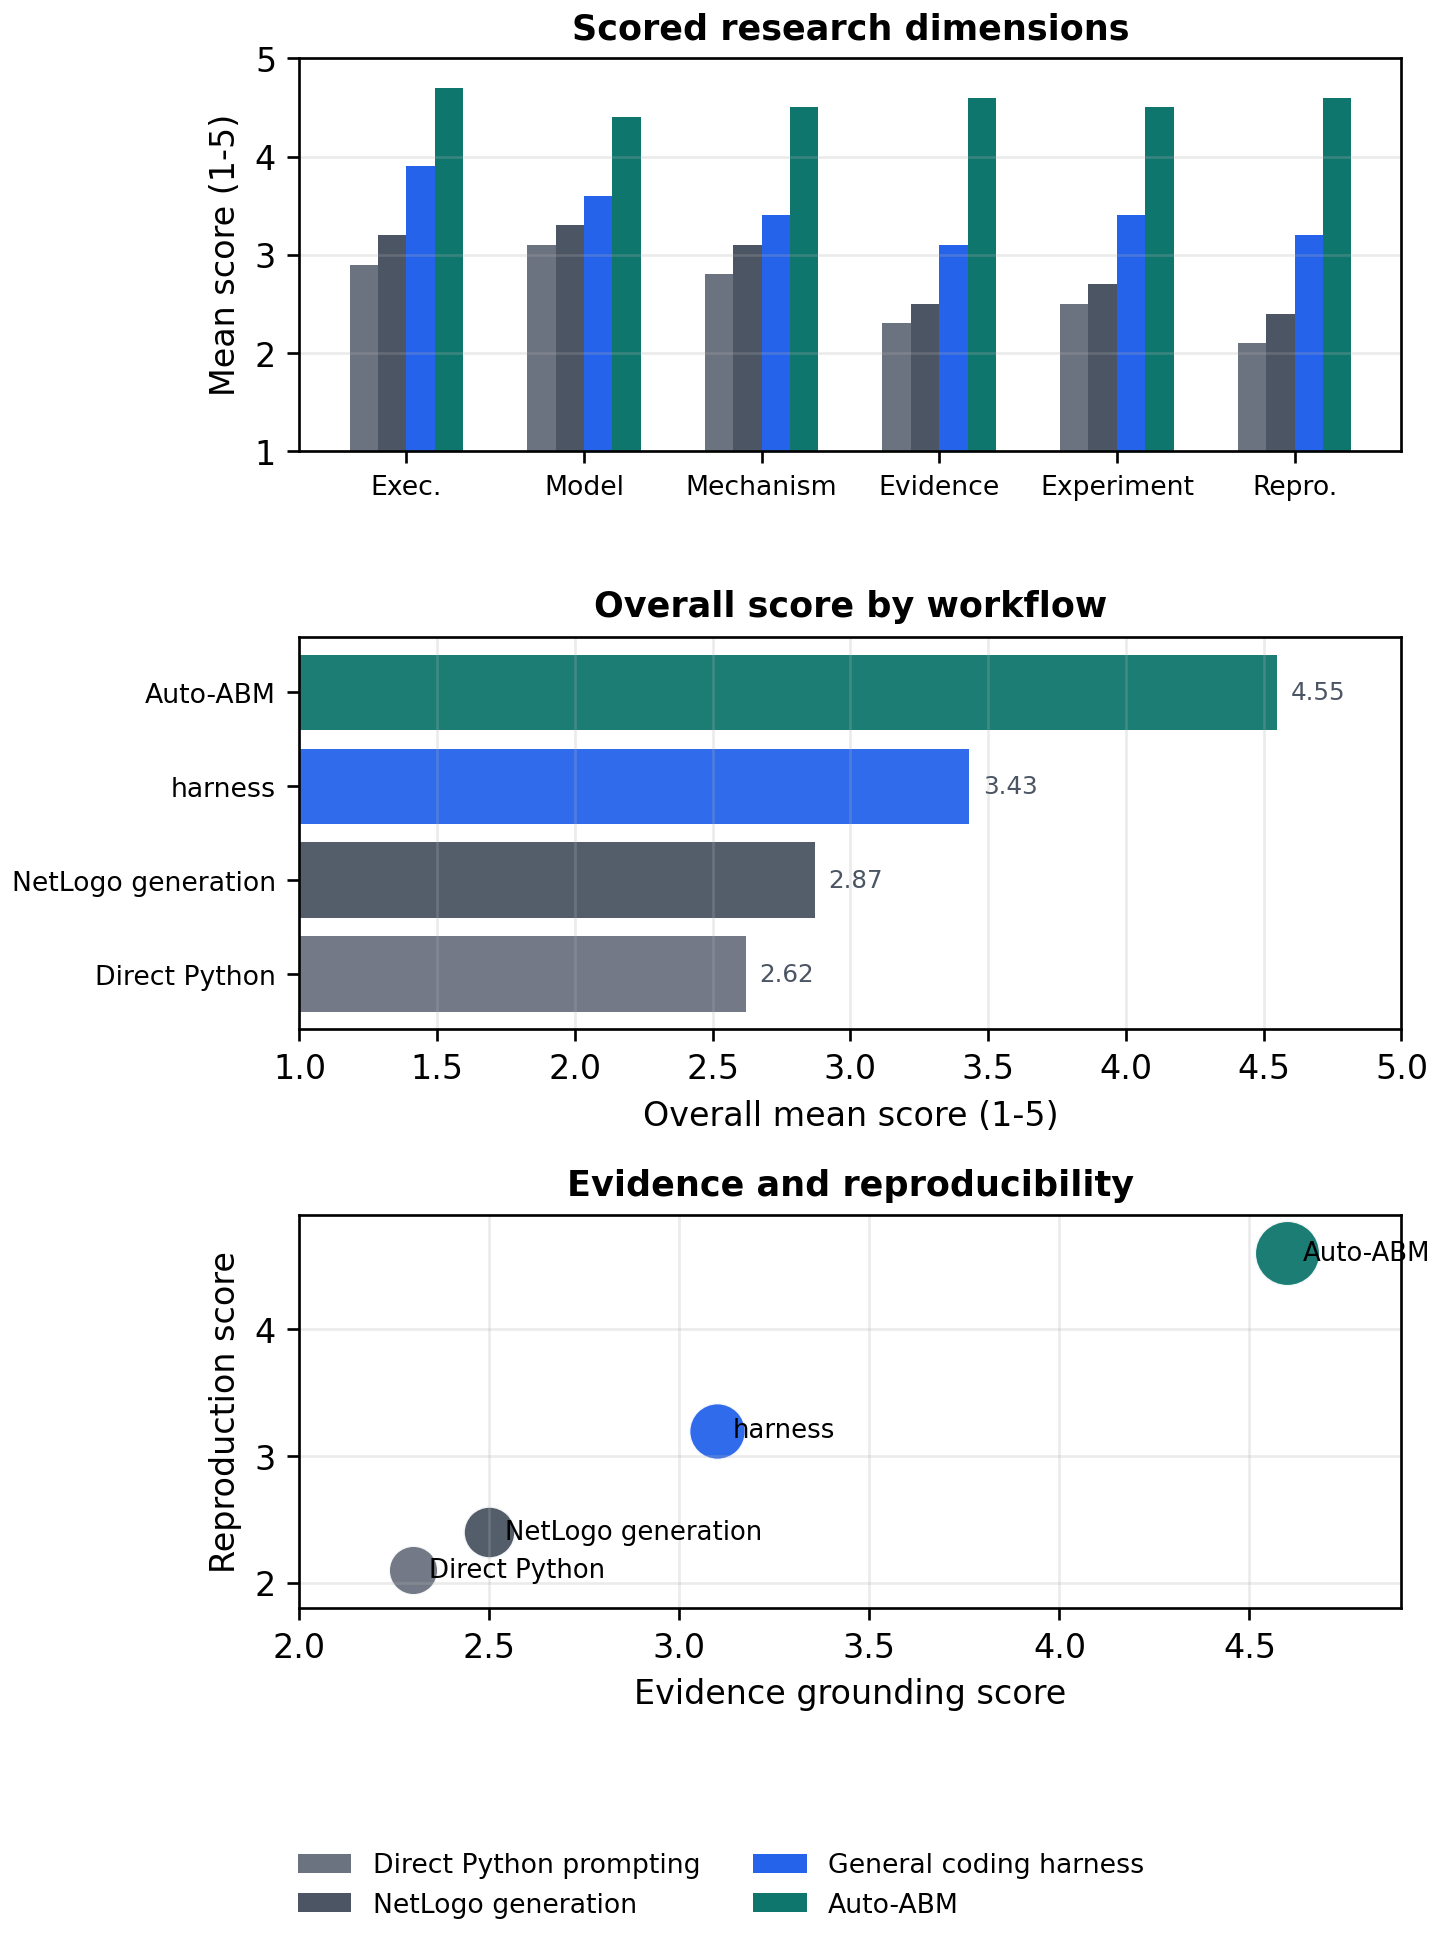
\includegraphics[width=\linewidth]{figures/fig-eval-dashboard.png}
  \caption{Draft result dashboard derived from Table~\ref{tab:main-results}. The panels compare score dimensions, overall averages, and the relationship between evidence grounding and reproduction completeness. Values are placeholders pending the controlled evaluation.}
  \label{fig:eval-dashboard}
\end{figure}

\section{Conclusion}
\label{sec:conclusion}

\sys{} reframes LLM-assisted ABM as a simulation-first research workflow. Rather than treating code generation as the endpoint, it keeps simulations, runs, traces, ODD documents, experiments, and exports as linked research objects. Its main contribution is the combination of specialized research agents, a deterministic Mesa kernel, a specification-derived mechanism atlas, evidence-checked explanations, and adaptive experiment views. The result is a workbench in which researchers can move from a question to a runnable model, inspect the evidence behind emergent behavior, and export a reproducible artifact from the same interface.

\section*{Limitations}

This draft describes a system that is still being prepared for final submission. The controlled evaluation is planned but not yet run, and the numeric results in Section~\ref{sec:evaluation} are placeholders. The current kernel covers common ABM families, but it is not a general simulator for every domain. The mechanism graph is derived from explicit specification references, so it may miss implicit dependencies hidden inside custom behavior implementations. Evidence validation checks cited trace facts, but it does not prove that the narrative interpretation is the only valid explanation. Autonomous exploration is implemented as a product direction and partial workflow, but the main evaluation should focus on the research-mode loop that is already end-to-end.

\section*{Ethics Statement}

\sys{} is intended to support modeling and interpretation, not to certify policy conclusions. ABM results depend on assumptions about agents, environments, and mechanisms. The workbench makes these assumptions more visible through ODD documents, trace evidence, and reproducible export, but users remain responsible for domain validation. Generated explanations should be treated as analytic summaries linked to trace evidence, not as causal proof outside the modeled system.

\bibliography{references}

\appendix

\section{Experiment Protocol Details}
\label{app:eval-protocol}

\begin{figure*}[t]
  \centering
  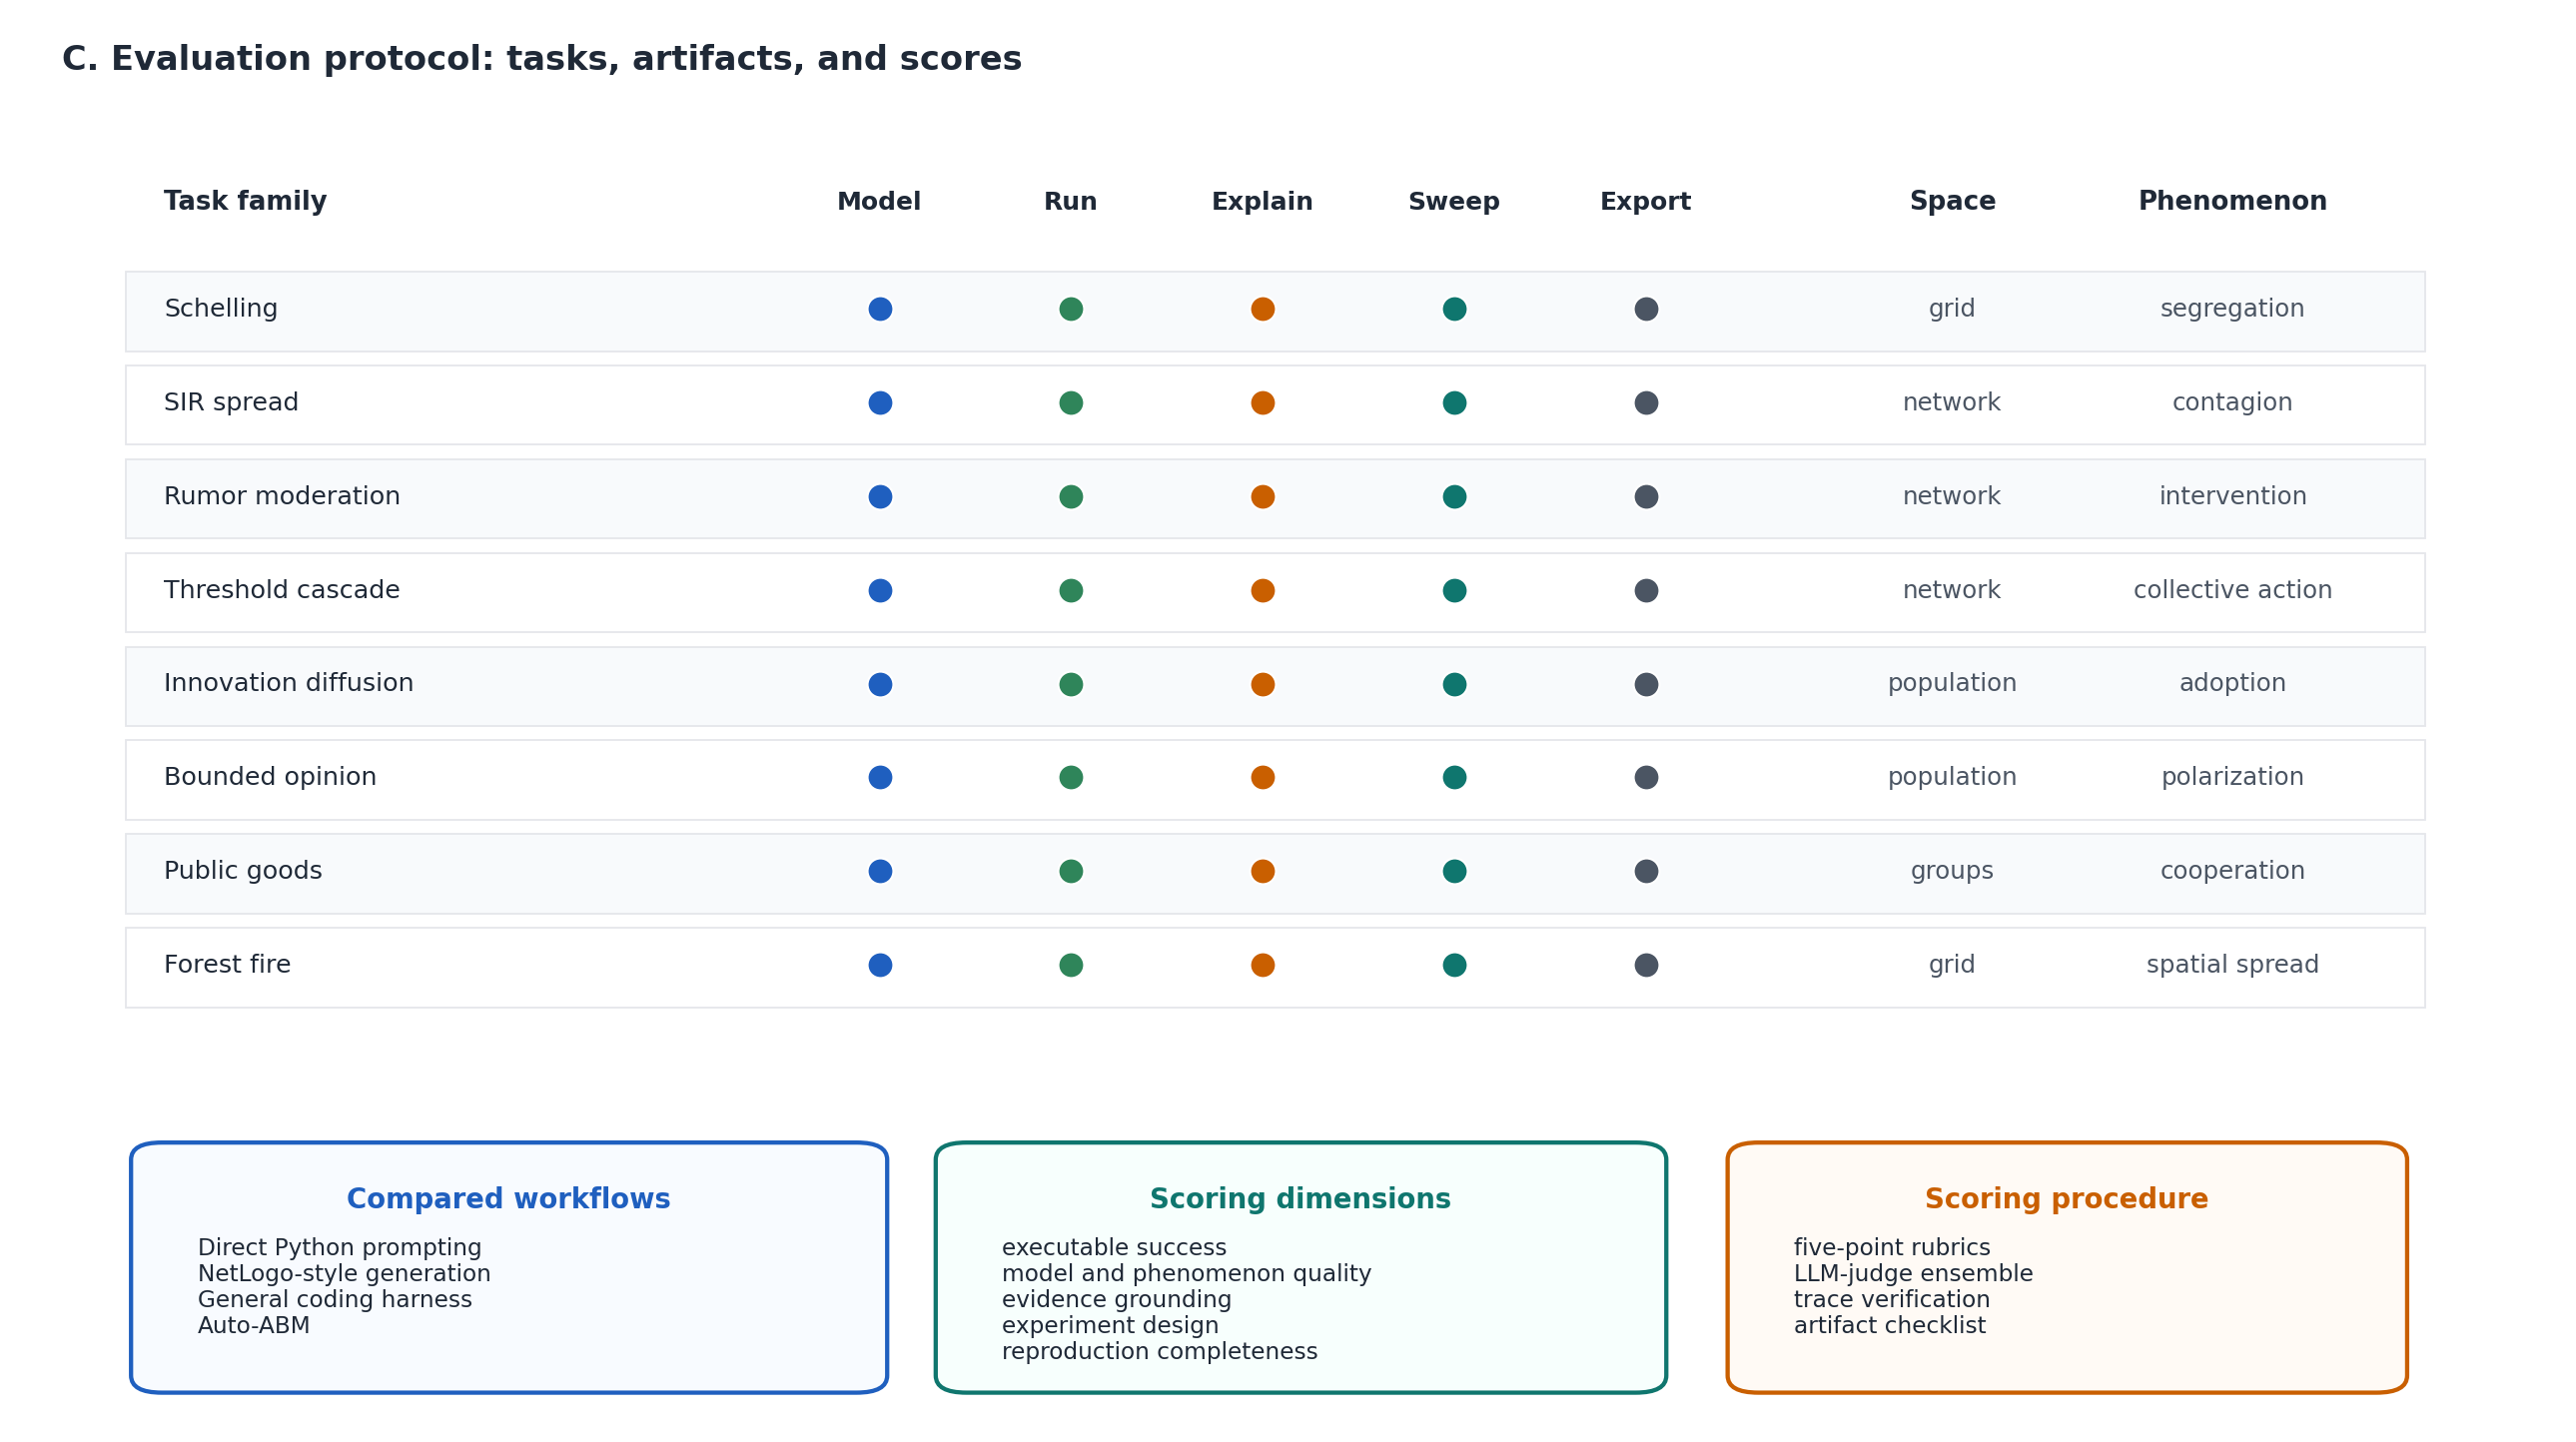
\includegraphics[width=0.98\textwidth]{figures/fig-eval-protocol.png}
  \caption{Planned experiment protocol. The task suite spans eight ABM families and five required artifacts. The same five-point scoring protocol is applied to every workflow and backend, covering executable validity, model quality, mechanism validity, evidence grounding, experiment quality, and reproduction completeness.}
  \label{fig:eval-protocol}
\end{figure*}

\section{Simulation Lifecycle Details}
\label{app:lifecycle}

\begin{table*}[t]
  \centering
  \small
  \begin{tabularx}{\textwidth}{p{0.13\textwidth}p{0.25\textwidth}YY}
    \toprule
    Stage & Coordinating role & Persistent objects & Evidence constraint \\
    \midrule
    Draft & Hypothesis agent & Candidate mechanisms, expected macro patterns, ODD rationale & Candidate curves are described as hypotheses until a run is executed. \\
    Formalize & Modeling agent & Versioned specification, parameter schema, synchronized ODD draft & Structural changes require validation and user approval. \\
    Execute & Execution agent & Run record, metric series, spatial snapshots, trace ledger & Only the kernel may create authoritative observations. \\
    Explain & Evidence agent and language narrator & Mechanism activity, attribution flows, cited explanation & Citations must match ticks, metrics, events, or mechanisms in the selected trace interval. \\
    Experiment & Experiment agent & Sweep design, intervention plan, resolved result panels & Charts are bound to recorded runs rather than generated values. \\
    Publish & Documentation agent & ODD document, reproduction package, provenance manifest & Export includes assumptions, seeds, run records, and integrity checks. \\
    \bottomrule
  \end{tabularx}
  \caption{Simulation-centered lifecycle in \sys{}.}
  \label{tab:lifecycle}
\end{table*}

\section{Research Role Catalogue}
\label{app:system-details}

\begin{table*}[t]
  \centering
  \small
  \begin{tabularx}{\textwidth}{p{0.22\textwidth}p{0.18\textwidth}Y}
    \toprule
    Research role & May mutate state & Primary responsibility \\
    \midrule
    Hypothesis agent & no & Propose mechanism families, expected macro patterns, and ODD-oriented rationales. \\
    Modeling agent & yes & Convert an adopted hypothesis into a validated simulation specification and versioned assumptions. \\
    Execution agent & yes & Submit the model to the deterministic kernel and preserve seed, parameter, and run provenance. \\
    Evidence agent & no & Transform trace intervals into mechanism activity, attribution flows, changepoints, and counterfactual summaries. \\
    Language narrator & no & Produce explanations only from evidence packets and mark unsupported statements as speculative. \\
    Experiment agent & yes & Design sweeps and interventions whose charts are bound to stored run records. \\
    Documentation agent & yes & Keep the ODD description, reproduction package, and provenance manifest aligned with the current simulation. \\
    \bottomrule
  \end{tabularx}
  \caption{Conceptual research roles used by \sys{}.}
  \label{tab:roles}
\end{table*}

\section{Trace and Export Contracts}
\label{app:contracts}

The kernel trace is an append-only record of run metadata, metric observations, events, mechanism firings, spatial snapshots, and termination status. Explanation modules read only the trace slice and record types needed for a selected interval. The export package contains the model specification, ODD document, experiment plans, run summaries, optional trace files, and a provenance manifest. The manifest records system version, kernel version, integrity checks, run identifiers, seeds, steps, parameter snapshots, model identity, and model version. This package is the object used to verify claims made about the submitted system.

\section{Per-Backend Score Estimates}
\label{app:backend-results}

\begin{table*}[t]
  \centering
  \small
  \begin{tabular}{llrrrr}
    \toprule
    Backend & Workflow & Overall & Model & Evidence & Repro \\
    & & (1--5) & (1--5) & (1--5) & (1--5) \\
    \midrule
    Claude Opus 4.6 & Direct Python & 2.75 & 3.2 & 2.5 & 2.3 \\
    Claude Opus 4.6 & NetLogo generation & 3.00 & 3.4 & 2.7 & 2.6 \\
    Claude Opus 4.6 & Harness & 3.60 & 3.8 & 3.3 & 3.4 \\
    Claude Opus 4.6 & \sys{} & 4.65 & 4.6 & 4.7 & 4.7 \\
    DeepSeek-V4 & Direct Python & 2.60 & 3.1 & 2.3 & 2.1 \\
    DeepSeek-V4 & NetLogo generation & 2.85 & 3.3 & 2.5 & 2.4 \\
    DeepSeek-V4 & Harness & 3.42 & 3.6 & 3.1 & 3.2 \\
    DeepSeek-V4 & \sys{} & 4.54 & 4.4 & 4.6 & 4.6 \\
    Qwen latest & Direct Python & 2.50 & 3.0 & 2.1 & 1.9 \\
    Qwen latest & NetLogo generation & 2.75 & 3.2 & 2.3 & 2.2 \\
    Qwen latest & Harness & 3.28 & 3.4 & 2.9 & 3.0 \\
    Qwen latest & \sys{} & 4.46 & 4.3 & 4.5 & 4.5 \\
    \bottomrule
  \end{tabular}
  \caption{Draft per-backend score estimates. These placeholder values are included to lock table shape before the real runs.}
  \label{tab:backend-results}
\end{table*}

\end{document}
